\documentclass[./\jobname.tex]{subfiles}
\begin{document}
%
\blindmathtrue
\blinddocument
%
\if\paper\FHVmode
	\section{Mathemodus}
\else
	\chapter{Mathemodus}
\fi
%
\begin{align}
\text{det}(\lambda \cdot \mathds{1} -A) &= 0 \underbrace{\longrightarrow}_{\substack{\text{Zustands-} \\ \text{rückführung}}} \text{det}\left[\lambda\cdot \mathds{1} - \left(A-b\cdot k\right)\right]=0\label{eq: eigenwerte rueckfuehrung}\\
\sin(x)^{2} + \cos(x)^{2} &= 1\label{eq: cos sin}
\end{align}
%
Ich bin eine super Referenzierung: \cref{eq: eigenwerte rueckfuehrung}. Oder noch besser wenn auf mehrere Gleichungen referenziert werden will: \cref{eq: eigenwerte rueckfuehrung,eq: cos sin}.
%
\if\paper\FHVmode
	\section{BiB \& Acronyme}
\else
	\chapter{BiB \& Acronyme}
\fi
%
\begin{itemize}
	\item Dies ist eine Qullenangabe: \parencite[Vgl.][S.220-224]{IEEE802.1Q2014}.
	\item Dies ist eine \gls{cbs}.
	\item Zweite Verwendung von einem Acronym: \gls{cbs}.
	\item Dies ist eine Fußzeile\footnote{Das ISO/OSI Model kann in \cite[][S.2-9]{Mandl2010} nachgeschlagen werden.}.
	\item \textcite[][S.2-9]{Mandl2010} nachgeschlagen werden.
\end{itemize}
%
So kann direkt Zitiert werden:
%
\begin{quote}
	\enquote{\textit{ich bin ein direktes Zitat}} \cite{Broster2001}
\end{quote}
%
Acronym Tests: \enquote{ \glspl{fpsLabel} \glspl{fpsLabel}} für Plural.
%
\newpage
%
\gls{tsn} \gls{jtag} \gls{sram} \gls{slam} \gls{bluecom} \gls{bluecom} \gls{profinet} \gls{ptp} \gls{bmca} \gls{dns} \gls{fpga} \gls{ack} \gls{bb} \gls{raspy} \gls{can} \gls{adc} \glspl{wlan} \gls{fft} \gls{fpu} \gls{bpsk} \gls{cgi}\par
%
\blindtext[1]
%
\if\paper\FHVmode
	\section{Bilder}
\else
	\chapter{Bilder}
\fi
%
In \autoref{fig: example-image} ist ein Beispiel einer Abbildung dargestellt.
%
\begin{figure}[H]
\centering
\noindent\adjustbox{max width=\linewidth}{% if the picture is greater than \textwidth, it is going to be resized to \textwidth.
	% trim option's parameter order: left bottom right top
	\includegraphics[width=1\textwidth]{example-image-a}
}
	% if you don't have to print the source, just remove it e.g.:
	%\unterschrift{ich bin die Unterschrift}{}{}
	% if you don't want to have your caption in the table of contents use the #3 argument to prevent the listing in the table of contents. e.q.:
	%\unterschrift{ich bin die Unterschrift}{Quelle}{no}
	\unterschrift{ich bin die Unterschrift}{Quelle}{}
	\label{fig: example-image}
\end{figure}
%
In \Cref{fig: Bild A,fig: Bild A} (oder mit Abkürzung \cref{fig: Bild A,fig: Bild A}) ist ein Beispiel einer Abbildung mit zwei Bildern dargestellt. \autoref{fig: Bild A und B} referenziert wiederum auf beide Bilder.
%
\begin{figure}[H]
	\centering
	\begin{subfigure}[b]{0.5\linewidth}
		\centering
		\includegraphics[width=1\textwidth]{example-image-a}
		\caption{Bild A}
		\label{fig: Bild A}
	\end{subfigure}% 
	%
	\begin{subfigure}[b]{0.5\linewidth}
		\centering
		\includegraphics[width=1\textwidth]{example-image-b}
		\caption{Bild B}
		\label{fig: Bild B}
	\end{subfigure}%
	\unterschrift{Bildunterschrift für beide Bilder}{\cite{Dorner2010}}{}%
	\label{fig: Bild A und B}
\end{figure}
%
\if\paper\FHVmode
	\subsection{Spezial}
\else
	\section{Spezial}
\fi
%
\def\spaceX{1.5}
\begin{figure}[H]
	\centering
	\noindent\adjustbox{max width=\linewidth}{
\begin{tikzpicture}%[scale=0.7]
\begin{scope}[every node/.style={bgelement}]
\node (Se) at (0,0) {Se};
\node[right=\spaceX of Se] (i) {1};
\node[above=\spaceX of i] (Iel) {$I:L_{a}$};
\node[below=\spaceX of i] (Rel) {$R:R_{a}$};
\node[right=\spaceX of i,label=below:{$\varPsi=k_{m}$}] (GY) {GY};
\node[right=\spaceX of GY] (w) {1};
\node[above=\spaceX of w] (Im) {$I:J_{m}$};
\node[below=\spaceX of w] (Rm) {$R:b_{m}$};
\end{scope}
\draw[bonds]
(Se) edge [e_out,effort={$U$}, flow={$i_a$}] (i)
(i) edge [e_out,effort={$U_{La}$}, flow={$i_a$}] (Iel)
edge [e_in,effort={$U_{Ra}$}, flow={$i_a$}] (Rel)
edge [e_in,effort={$U_{emf}$}, flow={$i_a$}] (GY)
(GY) edge [e_out,effort={$T$}, flow={$\omega$}] (w)
(w) edge [e_out,effort={$T_{j}$}, flow={$\omega$}] (Im)
edge [e_in,effort={$T_{b}$}, flow={$\omega$}] (Rm);
\end{tikzpicture}
}
	\unterschrift{Kausalisierter Bondgraph}{eigene Ausarbeitung}{}
\label{fig: kausalisierter bondgraph}
\end{figure}
%
\def\bildA{true}
\begin{figure}[H]
	\centering
	\noindent\adjustbox{max width=\linewidth}{%
	\subfile{./img/tikz/escon-schaltplan.tex}
}
	\unterschrift{Schaltkreis: Escon 50/5 Controller für Polverschiebung}{eigene Ausarbeitung}{}
	\label{fig: Schalplan Polverschiebung}
\end{figure}
%
\def\bildA{true}
\begin{figure}[H]
	\centering
	\noindent\adjustbox{max width=\linewidth}{%
		\subfile{./img/tikz/blockschaltbild-state-space.tex}
	}
	\unterschrift{Zustandsregler mit Rückkopplungsverstärkungsmatrix f}{eigene Ausarbeitung}{}
	\label{fig: blockschaltbild-state-space.tex A}
\end{figure}
%
\if\paper\FHVmode
	\section{Tabellen}
\else
	\chapter{Tabellen}
\fi
%
\begin{table}[H]
	\centering
	\noindent\adjustbox{max width=\linewidth}{
		\begin{tabular}{|c|c|c|c|c|c|c|c|c|c|}
			\hline
			\rowcolor[HTML]{\farbeTabA}
			Switch Typ & load & $n$ & min & max & $\tilde{x}$ & $\bar{x}$ & $\sigma^{2}$ & $\sigma$ \\ \hline
			Akro 6/0 & nein & 1199602 & 145.12 & 151.32 & 147.92 & 147.91 & 1.12 & 1.06	\\ \hline
			\rowcolor[HTML]{\farbeTabB} 
			Akro 6/0 & ja & 1199382 & 145.12 & 151.40 & 147.88 & 147.89 & 1.13 & 1.06 \\ \hline
		\end{tabular}
	}
	\unterschrift{Tabellen Unterschrift}{eigene Ausarbeitung}{}
	\label{tab: Tabelle A}
\end{table}
%
% Table with footnotes
%
\begin{table}[H]
	\centering
	\begin{threeparttable}
		\makebox[\linewidth]{%
			\begin{tabular}{c|p{5cm}}
				\hline
				\textbf{Typ} & \textbf{Eigenschaften}                                                                                                                                                                                                                                      \\ \hline
				Table 2 & \enquote{Fußnote}\tnote{a}\\\hline
				Table 2 & Fußnote\mtnote{b}\\\hline
				
			\end{tabular}}
		\unterschrift{Fußnoten in einer Tabelle}{eigene Ausarbeitun}{}
		\label{tab: Tabelle B}
		%
		\begin{tablenotes}
			\item [a] Diese Fußnote mit \enquote{\(\backslash\)tnote} nach \enquote{\(\backslash\)enquote} Umgebung verwenden
			\item [b] Ich bin die Fußnote zu b, für normalen Text.
		\end{tablenotes}
	\end{threeparttable}
	%
\end{table}
%
\if\paper\FHVmode
	\section{Listing}
\else
	\chapter{Listing}
\fi
%
\begin{lstlisting}[caption={example}]
for i:=maxint to 0 do
begin
	{ comment } %(*\label{comment}*)
end;
\end{lstlisting}
%
Line \ref{comment} shows a comment. Die Escape Operatoren können unter \enquote{./sty/Listings.sty} geändert werden. 
%
\if\paper\FHVmode
	\section{Todo List}
\else
	\chapter{Todo List}
\fi
%
\lipsum[1] 
\todo{This is a to do note at margin}
\lipsum[2] 
\todo[inline]{This is a todo note inline} 
\lipsum[3]
%
\if\paper\FHVmode
	\section{SVG Beispiel}
\else
	\chapter{SVG Beispiel}
\fi
%
\begin{enumerate}
	\item Installiere Inkscape
	\item Als erstes muss unter \enquote{Tools} \pfeil \enquote{Benutzer} \pfeil \enquote{SVG to PDF} die Konvertierung von SVG zu PDF gestartet werden. Dies sucht alle \enquote{.SVG} Dateien und wandelt diese zu \enquote{.PDF} Dateien um mit einer zusätzlichen Endung \enquote{-svg-raw.pdf}.\label{schritt translate}
	\item Anschließend kann das Dokument normal Übersetzt werden.
	\item Sind Änderungen an den SVG Dateien gemacht worden so muss \ref{schritt translate} ausgeführt werden.
\end{enumerate}
%
\begin{figure}[H]
	\centering
	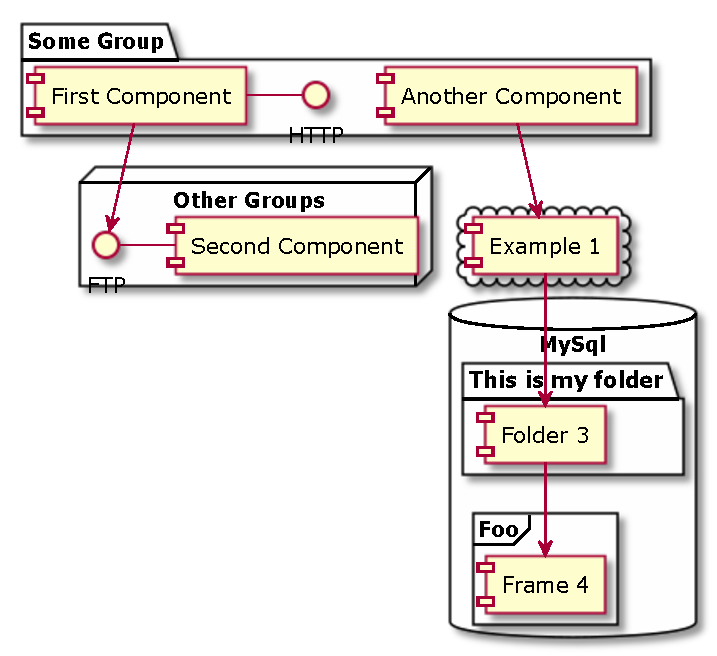
\includegraphics[width=0.75\linewidth]{./img/svg/Component_Diagram-test-svg-raw.pdf}
	\unterschrift{Beispiel für SVG}{eigene Ausarbeitung}{}
	\label{fig: beispiel svg}
\end{figure}
%
\if\paper\FHVmode
	\section{Algorithmen}
\else
	\chapter{Algorithmen}
\fi
%
Der \autoref{algo: first algo} ist gut.\par
%
\begin{algorithm}[H]
	\SetAlgoNoLine
	\DontPrintSemicolon
	\KwData{this text}
	\KwResult{how to write algorithm with \LaTeX2e }
	initialization\;
	\While{not at end of this document}{
		read current\;
		\eIf{understand}{
			go to next section\;
			current section becomes this one\;
		}{
			go back to the beginning of current section\;
		}
	}
	\unterschrift{How to write algorithms}{\url{https://en.wikibooks.org/wiki/LaTeX/Algorithms}}{}
	\label{algo: first algo}
\end{algorithm}
%
\if\paper\FHVmode
	\section{Referenzieren in den Anhang}
\else
	\chapter{Referenzieren in den Anhang}
\fi
%
\if\paper\FHVmode
	\subsection{test}
\else
	\section{test}
	\autoref{sec: test anhang}
\fi
%
\end{document}
